\chapter{System Analysis}

\subsection{System Requirement Specification}

General structure of a user story described in this document: 
\\ \\
\begin{normalsize}
\textbf{\{User story name\}}: As a \{role\}, I want \{goal\}, so that \{benefit\} (\{priority\}).
\end{normalsize}

\subsection{Functional Requirements}
The following sections describe the data required and the functional requirements that shall be performed in the new ERP System for both the HQ and field-based staffs.  These functional requirements include the on-going System maintenance and the creation and management reports for all areas.

\begin{itemize}
	\item The System shall have a common database core which allows integration of data and transactions between all financial, operational, production, and customer service functions within the ERP System.
	\item The System shall have a graphic user interface (GUI) implemented  as a Web-based interface
	\item The System shall be able to export selected records into either pdf or table file format
	\item The System shall have administrator ERP System and user security functionality to include:
		\begin{itemize}
			\item Setting Up a New User
			\item Updating an Existing User
			\item Restricting User Access to Certain Roles
		\end{itemize}
	\item The System shall have the ability for generated reports to be savable and exportable to numerous devices and mediums including printers
	\item The System shall produce Fixed Asset Depreciation Schedules
\end{itemize}

\subsection{Non-functional Requirements}

\paragraph{Reliability}
Reliability is the probability that the System will be able to process work correctly and completely without being aborted.
\\
The proposed ERP System has varying degrees of impact on areas of Stadia should parts of the System fail.
If the Core Systems functional areas of the System fail (becomes unusable) for a period of time the impact on Stadia would be as follows:

\begin{center}
\begin{table}[!hb]
\begin{tabular}{ | m{10em} | m{25em}| } 
  \hline
  \textbf{Length of Time of Outage} & \textbf{Impact to Stadia} \\ 
  \hline
   One Hour & Some Impact to {{TODO}} \\ 
   \hline
   One Day & Medium to Large Impact {{TODO}} \\
   \hline
   One Week & Very Large to Catastrophic Impact. \\
  \hline
\end{tabular}
\caption{Impact of reliablity on Stadia}
\end{table}
\end{center}

The minimum acceptable level of reliability for the core system Reporting aspect of the System would be no more than five (5) days (one work week).

\paragraph{Recoverability}
Recoverability is the ability to restore function and data in the event of a failure.

\begin{itemize}
	\item In the event the ERP application is completely unavailable to users (down) because of a System failure, it should be restored within 2 hours after the failure is detected.  This timeframe assumes that a locally controllable event (such as a hardware issue) has caused the outage.  If the application software is at issue and requires Contractor intervention, then the expected restoration time shall follow expected levels that shall be stated in the Service Level Agreement. 
	\item In the event that the operational database is corrupted, the database must be capable of being restored to its condition no more than 2 hours before the corruption occurred and must be restored to its most recent point in time prior to the corruption (1 day before). (Once a Contractor is selected a final data recovery strategy shall be determined).
\end{itemize}

The core system will perform periodic backups of all databases and will store these backups off-site.  At a minimum daily incremental changes to the database shall be captured and stored and on a weekly basis and a full database backup should be performed.  Daily backups shall be retained for at least six weeks (approximately one monthly close cycle) and weekly backups should be retained for at least fourteen weeks (one quarterly close cycle).  

In the event that the entire data center is destroyed, the following steps shall be required:
\begin{itemize}
	\item New Application and Database Servers would need to be located and installed
	\item Operating Systems shall need to be set up on the Servers(i.e Linux Server)
	\item Applications the ERP core System (Odoo) shall need to be installed on the Servers
	\item The last off-site back up of the ERP application database shall be restored to the Servers
\end{itemize}

\paragraph{System Availability}
System availability is the time when the application must be available for use. Required System availability is used in determining when maintenance may be performed.

The System must be available from 2:00 AM – 11:00 PM GMT+3 Monday – Saturday (National Holiday and Service Reduction Days not included).  Any scheduled down time for maintenance shall be not be scheduled around these core hours.

\paragraph{Fault Tolerance}
Not Applicable refer to Odoo Guideline

\paragraph{Performance}
The current preference is that accessing any transactional screen and updating data fields should take no more than 3 seconds.

System performance should be measured using up to 10 to 300 concurrent users(based on Stadia's number of employee)

\paragraph{Capacity}
The ERP System shall have the capacity to handle the types of volumes described below:
\begin{itemize}
	\item {TODO} number of employee creation per month
	\item {TODO} reports per month
\end{itemize}

\paragraph{Data Mapping and Conversion}
The following tables describe the data in the current system. he file structures and data in the current system are housed in Postgressql tables but are not truly relational in design.

\begin{itemize}
	\item A = Alphanumeric
	\item D = Date (MM/DD/YYYY)
	\item N = Numeric
\end{itemize}

\begin{center}
\begin{table}[!hb]
\begin{tabular}{|c|c|c|c|c| } 
  \hline
  \textbf{Ref} & \textbf{Description} & \textbf{Field Type} & \textbf{Note} & \textbf{Field Length (Bytes)} \\ 
  \hline
  1 & Badge ID & A & Generated Badge Number ID & 6 \\ 
  \hline
\end{tabular}
\caption{Datat mapping and conversion}
\end{table}
\end{center}


\paragraph{Design, Testing, Implementation, and Acceptance}
The Contractor/Provider shall be responsible for:

\begin{itemize}
	\item The design and configuration of the new ERP System based on Stadia business requirements.
	\item Installation of the ERP System in a test environment
	\item Loading the test database with sufficient data to perform the required User Acceptance Testing. This task shall be on-going until successful completion of the User Acceptance Testing. Both Stadia and Adarash will provide the User Acceptance Testing Matrix.
	\item Setup of the software and activation of the modules.
	\item Setup of the master files and tables and work with Stadia's staff to verify the data.
	\item Implementation of the ERP System into the final production environment.
	\item 
\end{itemize}

\paragraph{Training and Documentation}
The Contractor/Provider shall be responsible for:

\begin{itemize}
	\item Training of end users and technical staff to support to the ERP System to include:
		\begin{itemize}
			\item General Manger
			\item System Admin(IT staff)
			\item Clerks
			\item Department heads
		\end{itemize}
	\item Retraining for personnel as needed or requested by management
	\item Creating a learning team of "super users"(System Admins or IT staff) who can support others in all basic and some advanced functions
	\item Providing and/or creating training materials and technical documentation of the ERP System to include Quick Reference guides and an inmate self-learning module.
\end{itemize}

\section{System Requirement Analysis}

\subsection{Actor and Use Case Identification}
A use case diagram is a graphic depiction of the interactions among the elements of a system. A use case is a methodology used in the system analysis to identify, clarify, and organize system requirements in this context, the term \"system" refers to something being developed or operated such as a mail-order product sales and service website. Use case diagram are employed in UML (Unified Modeling Language). A standard notation for the modeling of real-world object and systems. System objectives can include planning overall requirements validating a hardware design, testing and debugging a software product under development, creating an online help reference, or performing a consumer-service oriented task. For example, use case in a product sales environment would include item ordering, catalog updating payment processing, and customer relations. A use case diagram contains four components.

\begin{figure}[!h]
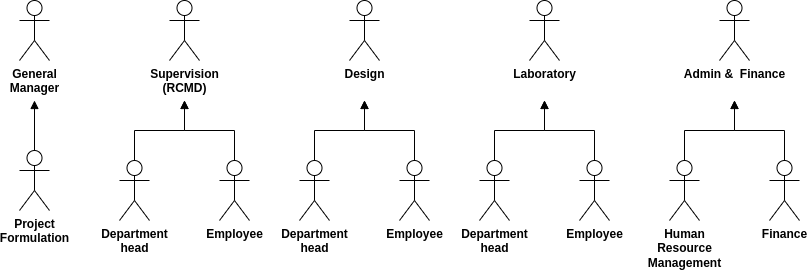
\includegraphics[width=13cm, keepaspectratio]{usecases/actors.png}
\label{shop_actors}
\caption{Actors involved }
\end{figure}

\subsection{Use Case Diagram}

Use case diagrams are used during the analysis
process to find system requirements and to design
system functionality. In this study use case
diagrams are used to describe the access rights of
each actor. Administrator Actors generally have a
function to manage users such as creating accounts
and setting access rights.

\subsubsection{Use Case Diagram And Description}
Website security requirements mandate separation of administrative interface from common functions provided to users. This segregation, for example, is strongly recommended by ISO 17799.

System should have separate application for administrators and for common users. It is recommended by OWASP Guide 2.0\footcite{https://www.owasp.org} that website administration application should not be accessible from  the internet without going through some management networks eg. via a strongly authenticated VPN or from a trusted network operation center.

Except for administrators, some part of the administrative interfaces should be also available to the Help desk staff (Customer Service) and some staffs, as they need to be able to assist customers having issues while using the customer oriented website.

Top level use case diagram below shows some administrative functions that administration website could provide.

%\paragraph{Top Level Use Case Diagram}
\begin{figure}[!hb]
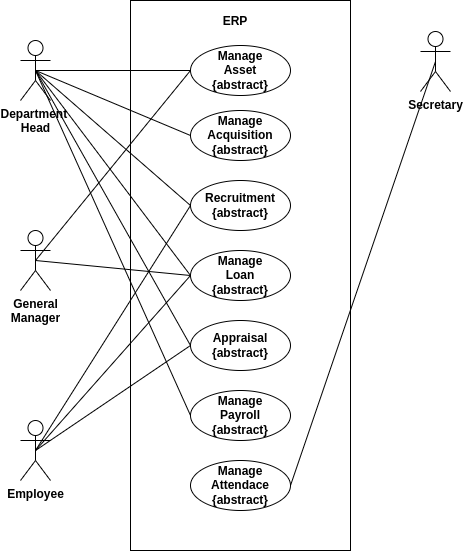
\includegraphics[width=15cm,keepaspectratio]{usecases/top_level_usecase.drawio.png}
\caption{Top level use case diagram}
\end{figure}
\clearpage

%################################# Mange Inventory #############################
\begin{figure}[!ht]
\centering
%\vspace*{-8cm}
%\hspace*{-3cm}
%\noindent
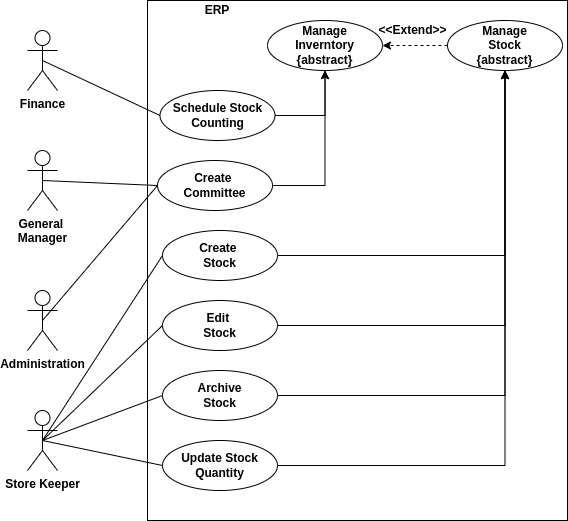
\includegraphics[width=15cm,keepaspectratio]{usecases/manage_inventory.drawio.png}
\caption{Manage Inventory use case diagram }
\end{figure}

\begin{table}[!h]
\begin{tabular}{|l|p{6cm}|p{6cm}|}
\hline 
\rule[-1ex]{0pt}{2.5ex} \textbf{Use Case Name} & \multicolumn{2}{p{10cm}|}{Manage Inventory} \\ 
\hline 
\rule[-1ex]{0pt}{2.5ex} \textbf{Description} &\multicolumn{2}{p{10cm}|}{Management of annual asset inventory in STADIA Engineering Works Consultant plc} \\ 
\hline 
\rule[-1ex]{0pt}{2.5ex} \textbf{Primary Actor}& \multicolumn{2}{p{10cm}|}{Finance, General 
Manager, Administration} \\ 
\hline 
\rule[-1ex]{0pt}{2.5ex} \textbf{Pre-Condition} & \multicolumn{2}{c|}{User has been logged on to system} \\ 
\hline 
\rule[-1ex]{0pt}{2.5ex} \textbf{Post-Condition} & \multicolumn{2}{p{10cm}|}{}  \\ 
\hline 
\multirow{4}{*}{\textbf{Basic Flow}} & \textbf{Actor Action} & \textbf{System Response}\\
\cline{2-3}
%
&
\textbf{1.}  The Use Case starts when the user is logged on to the website and select the manage inventory menu.
& 
\textbf{2.}  The system will display lists of assets.
\\
%
&
\textbf{3.}  The user will Schedule stock counting in calendar.
& 
\textbf{4.}  The system will set and notify other depertments. 
\\
%
&

& 
\textbf{5.}  The Use Case ends. 
\\
\hline 
\rule[-1ex]{0pt}{2.5ex} \textbf{Alternate Flow} & \multicolumn{2}{p{10cm}|}{\textbf{A1 : } If the user requests to create commitee:}  \\ 
\cline{2-3}
\multirow{2}{*}{} & \textbf{Actor Action} & \textbf{System Response}\\
\cline{2-3}
%
&
\textbf{2.1}  The user click create commite button/icon the scheduled stock counting date. 
& 
\textbf{2.2}  The system display a form for selecting stock counting commite. 
\\
%
&
\textbf{2.3}  The user fills out the and submit the form. 
& 
\textbf{2.4}  The Use Case ends.  
\\
\hline
\end{tabular}
\caption{Manage inventory} 
\end{table}

%--------------------Stock
\begin{table}[!h]
\begin{tabular}{|l|p{6cm}|p{6cm}|}
\hline 
\rule[-1ex]{0pt}{2.5ex} \textbf{Use Case Name} & \multicolumn{2}{p{10cm}|}{Manage Stock} \\ 
\hline 
\rule[-1ex]{0pt}{2.5ex} \textbf{Description} &\multicolumn{2}{p{10cm}|}{The idea is that user could create different stocks, modify and remove} \\ 
\hline 
\rule[-1ex]{0pt}{2.5ex} \textbf{Primary Actor}& \multicolumn{2}{p{10cm}|}{Store Keeper} \\ 
\hline 
\rule[-1ex]{0pt}{2.5ex} \textbf{Pre-Condition} & \multicolumn{2}{c|}{User has been logged on to system} \\ 
\hline 
\rule[-1ex]{0pt}{2.5ex} \textbf{Post-Condition} & \multicolumn{2}{p{10cm}|}{}  \\ 
\hline 
\multirow{4}{*}{\textbf{Basic Flow}} & \textbf{Actor Action} & \textbf{System Response}\\
\cline{2-3}
%
&
\textbf{1.}  The Use Case starts when the user is logged on to the website and manage inventory stock.
& 
\textbf{2.}  The system will display lists of assets.
\\
%
&
\textbf{3.}  The user will select create new asset.
& 
\textbf{4.}  The system will display form for creating new asset. 
\\
%
&
\textbf{5.}  The user will fill the displayed from and submit the form.
& 
\textbf{6.}  The system will verify the information like if the data is redundant or not and store the asset information. 
\\
%
&

& 
\textbf{7.}  The Use Case ends. 
\\
\hline 
\rule[-1ex]{0pt}{2.5ex} \textbf{Alternate Flow} & \multicolumn{2}{p{10cm}|}{\textbf{A1 : } If the user requests to edit an existing asset:}  \\ 
\cline{2-3}
\multirow{2}{*}{} & \textbf{Actor Action} & \textbf{System Response}\\
\cline{2-3}
%
&
\textbf{2.1}  The user click edit button/icon for the selected asset. 
& 
\textbf{2.2}  The system display the same form as creating new asset, but filled with the selected asset information. 
\\
%
&
\textbf{2.3}  The user edits the options and submit the form. 
& 
\textbf{2.4}  The flow continues to Basic flow 6  
\\
\hline
\end{tabular}
\caption{Manage Stock} 
\end{table}

%################################# End Mange Inventory ############################# 

%################################# Asset ############################# 
\clearpage
\begin{figure}[!ht]
\centering
%\vspace*{-8cm}
%\hspace*{-3cm}
%\noindent
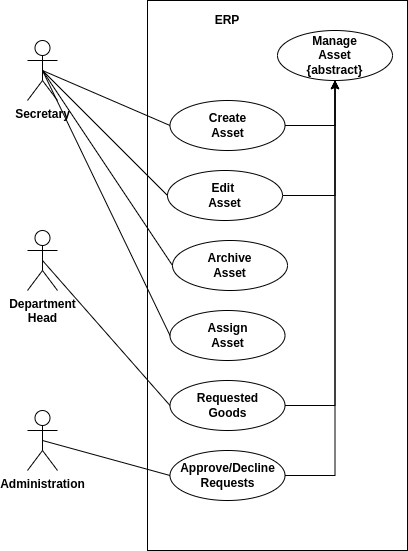
\includegraphics[width=10cm,keepaspectratio]{usecases/asset.drawio.png}
\caption{Manage Acquisition use case diagram }
\end{figure}

%--------------------Asset
\begin{table}[!h]
\begin{tabular}{|l|p{6cm}|p{6cm}|}
\hline 
\rule[-1ex]{0pt}{2.5ex} \textbf{Use Case Name} & \multicolumn{2}{p{10cm}|}{Manage Asset} \\ 
\hline 
\rule[-1ex]{0pt}{2.5ex} \textbf{Description} &\multicolumn{2}{p{10cm}|}{Good issuance
and Return procedure} \\ 
\hline 
\rule[-1ex]{0pt}{2.5ex} \textbf{Primary Actor}& \multicolumn{2}{p{10cm}|}{Store Keeper} \\ 
\hline 
\rule[-1ex]{0pt}{2.5ex} \textbf{Pre-Condition} & \multicolumn{2}{c|}{User has been logged on to system} \\ 
\hline 
\rule[-1ex]{0pt}{2.5ex} \textbf{Post-Condition} & \multicolumn{2}{p{10cm}|}{}  \\ 
\hline 
\multirow{4}{*}{\textbf{Basic Flow}} & \textbf{Actor Action} & \textbf{System Response}\\
\cline{2-3}
%
&
\textbf{1.}  The Use Case starts when the user is logged on to the website and manage inventory stock.
& 
\textbf{2.}  The system will display lists of assets.
\\
%
&
\textbf{3.}  The user will select request good.
& 
\textbf{4.}  The system will notify store keeper. 
\\
%
&

& 
\textbf{5.}  The Use Case ends. 
\\
\hline
\end{tabular}
\caption{Manage Stock} 
\end{table}

%################################# End Of Asset ############################# 


%################################# Acquisition #############################
\begin{figure}[!ht]
\centering
%\vspace*{-8cm}
%\hspace*{-3cm}
%\noindent
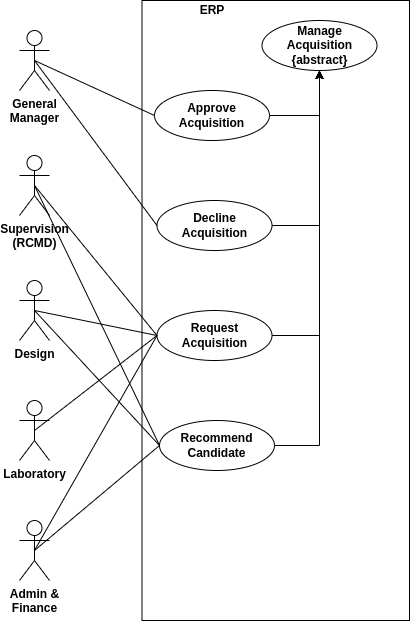
\includegraphics[width=10cm,keepaspectratio]{usecases/acquisition_usecase.drawio.png}
\caption{Manage Acquisition use case diagram }
\end{figure}
%################################# End Of Acquisition############################# 

%################################# Recruitment #############################
\begin{figure}[!ht]
\centering
%\vspace*{-8cm}
%\hspace*{-3cm}
%\noindent
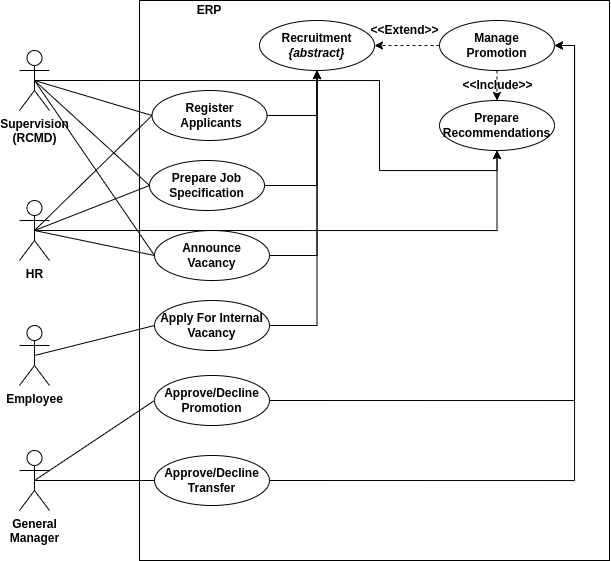
\includegraphics[width=15cm,keepaspectratio]{usecases/recruitment.drawio.png}
\caption{Manage Recruitment use case diagram }
\end{figure}
%################################# End Of Recruitment ############################# 


%################################# Loan #############################
\begin{figure}[!ht]
\centering
%\vspace*{-8cm}
%\hspace*{-3cm}
%\noindent
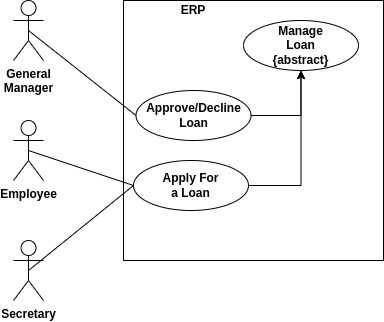
\includegraphics[width=10cm,keepaspectratio]{usecases/loan.drawio.png}
\caption{Manage Loan use case diagram }
\end{figure}
%################################# End Of Loan ############################# 

%################################# appraisal #############################
\begin{figure}[!ht]
\centering
%\vspace*{-8cm}
%\hspace*{-3cm}
%\noindent
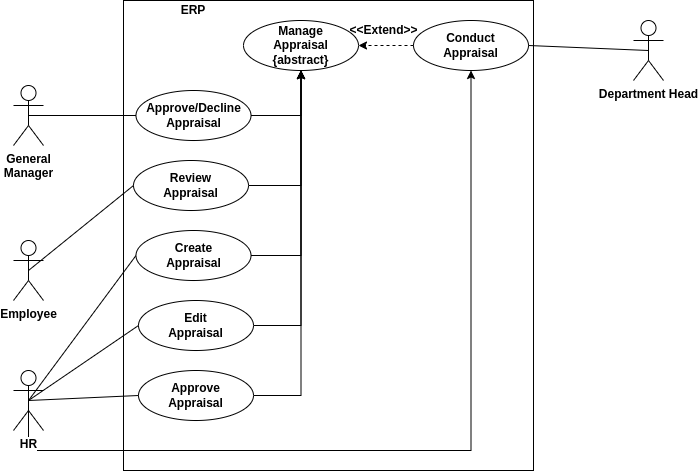
\includegraphics[width=15cm,keepaspectratio]{usecases/appraisal.drawio.png}
\caption{Appraisal use case diagram }
\end{figure}
%################################# End Of appraisal ############################# 


%################################# Payroll #############################
\begin{figure}[!ht]
\centering
%\vspace*{-8cm}
%\hspace*{-3cm}
%\noindent
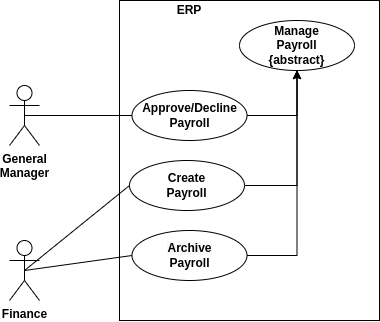
\includegraphics[width=10cm,keepaspectratio]{usecases/payroll.drawio.png}
\caption{Manage Payroll use case diagram }
\end{figure}
%################################# End Of Payroll ############################# 



\begin{figure}[!ht]
\centering
%\vspace*{-8cm}
%\hspace*{-3cm}
%\noindent
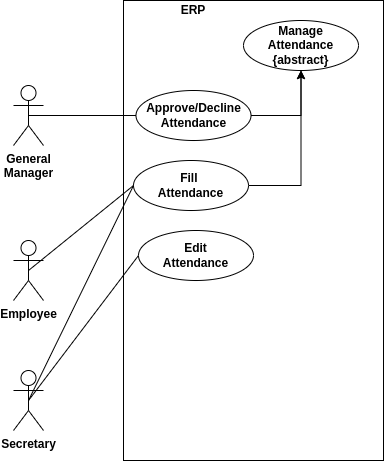
\includegraphics[width=10cm,keepaspectratio]{usecases/attendance.drawio.png}
\caption{Manage Attendance use case diagram }
\end{figure}
%################################# End Of Attendacne ############################# 

\clearpage

%\subsubsection{Administrator Use Case Diagram}

%\subsubsection{Manager Use Case Diagram}

%\subsubsection{HR Use Case Diagram}

%\subsection{Activity Diagram}

%\subsubsection{Recruitment Module Activity Diagram}

%\subsubsection{Human Resources Activity Diagram}

%\subsubsection{Attendance Activity Diagram}

%\subsubsection{Leave (time off) Activity Diagram}

%\subsubsection{Payroll Activity Diagram}

%\subsubsection{Performance Management (Appraisal) Activity Diagram}

%\subsubsection{Asset Management Activity Diagram}


%\subsection{User Access Rights}

%\hspace{-2cm}
%\begin{tabularx}{540pt}{|X|c|c|c|c|c|c|c|p{3cm}|}

%{|*{9}{Y|}}

%\hline

%\textbf{No} & \textbf{User} & \textbf{Acess Level} & \textbf{Object} & \multicolumn{4}{c|}{\textbf{Acess Right}} & \textbf{Information} \\
%\cline{5-8} & &  &  & Read & Write & Create & Delete & \\

%\hline

%\multirow{1}{*}{1} & \multirow{1}{*}{Administrator} & \multirow{1}{*}{Administration} & ALL & \cmark & \cmark & \cmark & \cmark & Top Level \\

%\hline

%\multirow{2}{*}{2} & \multirow{2}{*}{System Admin} & \multirow{2}{*}{System Admin} & 
%User & \cmark & \cmark & \cmark & \xmark & Second level below Administrator \\
%\cline{4-8} & & & 
%Acess Right 2 & \xmark & \xmark & \xmark & \xmark & \\

%\hline

%\multirow{2}{*}{3} & \multirow{2}{*}{Manager} & \multirow{2}{*}{Manger} & 
%Attendance & \cmark & \cmark & \xmark & \xmark & Manager \\
%\cline{4-8} & & & 
%Acess Right 2 & \xmark & \xmark & \xmark & \xmark & \\

%\hline

%\end{tabularx}
%\hspace*{-1cm}

\clearpage
\subsection{Activity Diagram}
Are graphical representations of workflows of stepwise activities and actions with support for choice, iteration and concurrency. In the Unified Modeling Language, activity diagrams are intended to model both computational and organizational processes (i.e., workflows), as well as the data flows intersecting with the related activities. Although activity diagrams primarily show the overall flow of control, they can also include elements showing the flow of data between activities through one or more data stores.\footcite{wikiactivitydiagram}

%\subsubsection{Action States and Activity States}
%\begin{itemize}
%	\item Action states are atomic and cannot be decomposed
%	\item Work of the action state is not interrupted.
%	\item Activity states can be further decomposed
%	\item Their activity being represented by other activity diagrams
%	\item They may be interrupted
%	\item Represented in UML by a rounded rectangle.
%	\item Activity represents the performance of some behavior in the work flow.
%\end{itemize}

\begin{figure}[!h]
\label{login_activity_diagram}
\center
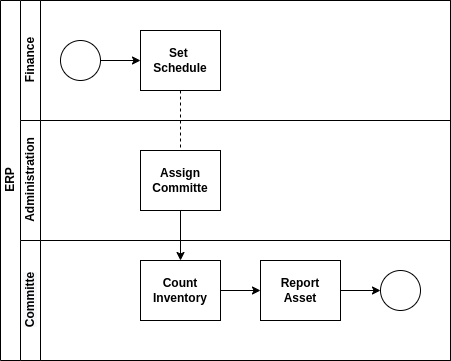
\includegraphics[width=10cm,keepaspectratio]{activity_diagrams/manage_inventory_activity_diagram.drawio.png}
\caption{Invenory activity diagram}
\end{figure}


\begin{figure}[!h]
\label{asset_activity_diagram}
\center
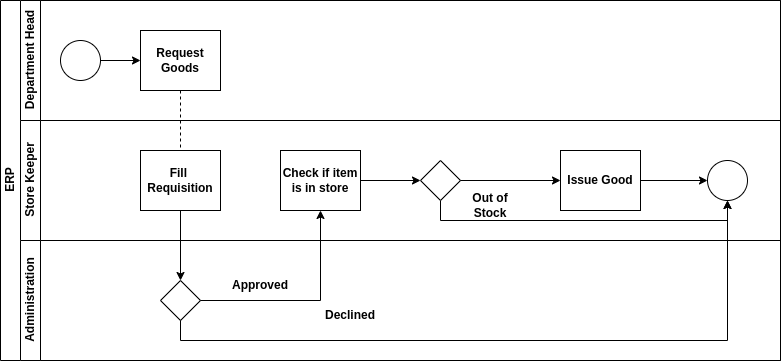
\includegraphics[width=15cm,keepaspectratio]{activity_diagrams/manage_asset_activity_diagram.drawio.png}
\caption{Issue asset activity diagram}
\end{figure} 

\begin{figure}[!h]
\label{loan_activity_diagram}
\center
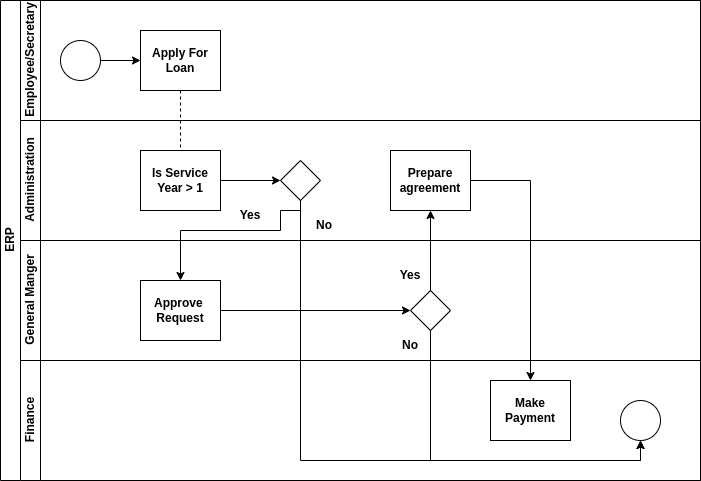
\includegraphics[width=15cm,keepaspectratio]{activity_diagrams/loan_activity_diagram.drawio.png}
\caption{Loan activity diagram}
\end{figure}

\begin{figure}[!h]
\label{loan_activity_diagram}
\center
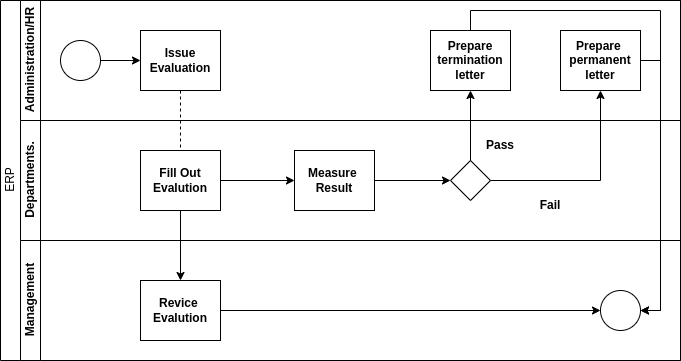
\includegraphics[width=15cm,keepaspectratio]{activity_diagrams/appraisal_activity_diagram.drawio.png}
\caption{Performance Evaluation activity diagram}
\end{figure}